\documentclass[a4paper,12pt]{report}
\usepackage{graphicx}
\usepackage{booktabs}
\usepackage{amsmath}
\usepackage{listings}
	\title{Scilab Identification Toolbox - Existing features}
\begin{document}
	

	
\maketitle
	\tableofcontents		
	
	
\chapter{Calling Sequence}	
	\lstinputlisting{call.sci}	
%		\begin{figure}[tbp]
%		\centering
%		\includegraphics[width=0.8\textwidth]{codeSci.JPG}
%		\caption{Calling Sequence}
%		\label{}
%	\end{figure}
	
\chapter{Model structure (idpoly)}
	
	\section{Model structure output}
	\begin{enumerate}
		\item Model representation (A,B,C polynomials in increasing power of $z^{-1}$)
		
	\item  Sampling time 
	\item Performance of model - Values of Mean Squared Error(MSE), Final Prediction Error(FPE), Fit Percentage, Raw Akaike's Information Criterion(AIC), Small sample-size corrected (AICc), Normalized AIC(nAIC), Bayesian information criteria(BIC)
	\end{enumerate}
\section{Model structure attributes}
\begin{enumerate}
	\item Polynomial coefficients vector
	\item Variable('$z^{-1}$') used in polynomials
	\item Time unit
	\item Smpling time
	\item Report giving values of MSE, FPE, Fit Percentage, AIC, AICc, AICn, BIC
\end{enumerate}
	

	
	\begin{figure}[tbp]
		\centering
		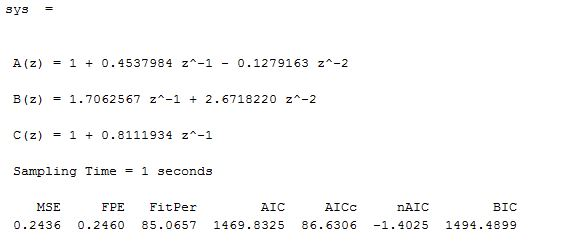
\includegraphics[width=0.8\textwidth]{modSci1.JPG}
		\caption{Model(idpoly) Output}
		\label{}
	\end{figure}
	
	\begin{figure}[tbp]
		\centering
		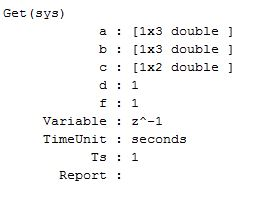
\includegraphics[width=0.8\textwidth]{modSci2.JPG}
		\caption{Model attributes}
		\label{}
	\end{figure}
	
	\chapter{Data structure (iddata)}
	
	\section{Data structure output}
	\begin{enumerate}
		
		\item Domain of data : Time (No provision of storing frequency domain data in iddata. Another function 'frd' can store frequency and response data)
		\item Number of samples
		\item Name of output data vector 
		
		\item Name of input data vector
		
		\item Sampling time
		
	\end{enumerate}
	Note : No provision of changing name of output or input data vector and time unit.
	\section{Data struture attributes}
		
	\begin{enumerate}
		\item Output data vector 
		
		\item Input data vector
		
		\item Sampling time
		
		\item Time unit
	\end{enumerate}

	
			\begin{figure}[tbp]
			\centering
			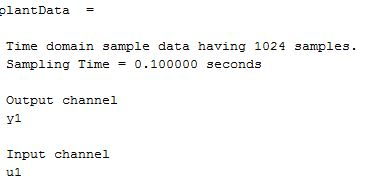
\includegraphics[width=0.8\textwidth]{datSci1.JPG}
			\caption{Data(iddata) Output}
			\label{}
		\end{figure}
	
			\begin{figure}[tbp]
			\centering
			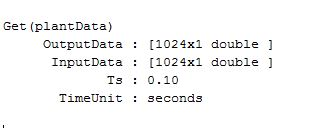
\includegraphics[width=0.8\textwidth]{datSci.JPG}
			\caption{Data attributes}
			\label{}
		\end{figure}
		
	\chapter{Optimizer}
	\begin{enumerate}
		
		\item diffcode toolbox - Automatic differentiation (consists of functions to evaluate jacobian and hessian but no associated optimizer)
		\item Optimbase toolbox - building block for optimization methods(number of variables, minimum and maximum bounds, number of non linear inequality constraints, cost function, logging system, various termination criteria)
		
		\item Nonlinear Least Squares
		\begin{enumerate}
	     	\item lsqrsolve - Levenberg-marquardt algorithm (used in arx, armax, oe) 
		
		\item leastsq - Non-linear least squares problem 
		
		Algorithms available : quasi-Newton (default), conjugate gradient or non-differentiable
	
		
		
		
		\item datafit - Parameter identification based on measured data
		
	Algorithms available : quasi-Newton (default), conjugate gradient or non-differentiable
		
		
	\end{enumerate}
	\item optim - Non-linear optimization
		
		Algorithms available : limited memory BFGS algorithm, quasi-Newton method, non-differentiable problems
		
		
		\item karmarkar - Constrained linear optimization problem
		
		
		\item neldermead - Direct search optimization algorithms based on the simplex method
		
	\item qpsolve - Quadratic optimization (active set)
		
	\item Ipopt - Interior point method
		
		\item conjgrad - Conjugate gradient solvers
	\end{enumerate}
	
	
	
	
	
	
\end{document}